\chapter{Anforderungsanalyse}
\label{chap:anforderungsanalyse}
    Dieses Kapitel befasst sich im Allgemeinen mit der Anforderungsanalyse und -erhebung. Hierbei wird eine
    Marktanalyse repräsentiert, um das Potential rundum \acl{SH} aufzuzeigen und ein Gefühl 
    dafür zu vermitteln, welche Anforderungen dabei entstehen können, bzw. bereits bestehen. Die Analyse ist 
    mit repräsentativen Statistiken, Studien und Umfragen belegt. Hauptsächlich wird im Rahmen der Anforderungserhebung 
    auf die Methodiken und Techniken eingegangen, die verwendet werden, um 
    Anforderungen zu identifizieren. Diese dienen als Grundlage für die Konzeption der Steuerzentrale. Bestandteile der 
    Anforderungserhebung sind unter anderem zentrale Prozesse des \acl{RE}, ein \textit{user-centered Design}, im Deutschen 
    nutzerzentriertes Design, eine \textit{Target Group Analysis}, im Deutschen Zielgruppenanalyse, und die Durchführung von 
    Experteninterviews. Diese Interviews sind nicht repräsentativ und dienen lediglich der weiträumigeren Informationsgewinnung. 
    \\
    Vorab wird sichergestellt, dass im Rahmen des benutzerzentrierten Designs der Softwareentwickler als Nutzer und Anwender im 
    Vordergrund steht, da dieser die Plattform betreibt, bzw. für die Erweiterung der Software als auch für die 
    Anpassungen auf die eigenen Anwendungsfälle zuständig ist.
    \\
    \linebreak
    Damit ein Eindruck entsteht, welches Marktpotential \acl{SH} Anwendungen haben und welche Anforderungen somit 
    verbunden sind, wird basierend auf gegebenen Studien, Statistiken und Umfragen eine Marktanalyse durchgeführt.

\section{Marktanalyse}
\label{sec:marktanalyse}
    Der Markt rundum \acl{SH} nimmt immer weiter zu. Sei es die Entwicklung von neuen intelligenten Geräten, die 
    Massentauglichkeit von Geräten %, die nicht lange am Markt bestehen 
    oder die stetig wachsende Abdeckung von Anwendungsfällen und Übernahme von Aufgaben und Prozessen. Durch die Vielzahl an 
    Produktanbietern und diversen Kommunikationsmöglichkeiten, ist es schwierig eine Lösung für alle Alternativen und 
    Produktausprägungen anzubieten. Hersteller versuchen mit der angebotenen Produktpalette ihr eigenes Ökosystem im Bereich 
    \acl{SH} zu erstellen, um die Nutzer abhängig zu machen. Der repräsentativen Studie von Deloitte zufolge ist jedoch eine 
    Insellösung bei den Nutzern in Deutschland nicht gefragt \cite{deloitte2018}. Befragt wurden 2000 Konsumenten zwischen 
    19 und 75 Jahren. Einem geringen Anteil von 22 Prozent der 
    Befragten ist die Erweiterbarkeit des Systems mit Produkten anderer Hersteller weniger, bzw. nicht wichtig. Im Gegensatz dazu 
    empfinden 43 Prozent der Befragten die Erweiterbarkeit als wichtig und 28 Prozent als sehr wichtig \cite{deloitte2018}. 
    Demnach müssen die Hersteller eine flexiblere Einsetzbarkeit gewährleisten, damit solche Systeme den Marktdurchbruch 
    erlangen. Dadurch wird die Entwicklung von Plattformen komplexer und umfangreicher. Beispielsweise sind die am weit 
    verbreitetsten Open Source Plattformen, openHAB und Home Assistant, sehr komplex und bilden ein großes Ökosystem ab, da 
    stetig der Zuwachs an integrierbaren Geräten zunimmt und damit der Funktionsumfang steigt.  

    \subsection{Allgemeine Marktsituation und Marktprognose}
    %Anbieter, Plattformen, Geräte
        Derzeit gibt es viele Anbieter für intelligente Produkte. Diese bieten zum einen einzelne Geräte an, die in 
        beliebige Plattformen integriert werden können und zum anderen ein eigenes Ökosystem, sofern der Anwender 
        mehrere Produkte des Anbieters nutzen möchte. Dennoch ist in den meisten Fällen die Konfiguration der Geräte nur auf 
        den hauseigenen Plattformen möglich. Somit kann der Nutzer nicht alle Komponenten ausschließlich über eine Plattform 
        konfigurieren und steuern. 
        \\
        \linebreak
        Eine repräsentative Umfrage der \ac{SGCS} mit 1384 Teilnehmern, welche im April 2022 veröffentlicht wurde, zeigt, welche 
        Anbieter in Deutschland am meist verbreitetsten sind, bzw. welche die Nutzer am häufigsten kaufen. An oberster Stelle 
        steht Philips und Samsung mit jeweils 25 Prozent und an dritter Stelle Bosch mit 23 Prozent. Weitere Anbieter können dem 
        Diagramm im Anhang (siehe \ref{appendix:brandings}) entnommen werden. Dabei sind jedoch weitaus nicht alle Hersteller und 
        Anbieter aufgelistet. Detaillierter wird an dieser Stelle jedoch nicht eingegangen. 
        \\
        \linebreak
        Der aktuelle Markt für intelligente Produkte ist in sechs primäre Segmente aufgeteilt, die jeweils andere Anwendungsfälle 
        abdecken \cite{statista2021}:
        \begin{itemize}
            \item Kontrolle und Konnektivität: Gateways die alle Geräte jeglicher Segmente kontrollieren, intelligente Lautsprecher 
            mit dem Fokus zur Kontrolle und der digitalen Unterstützung und bspw. intelligente Steckdosen
            \item Intelligente Geräte (Smart Appliances): Kühlschrank, Waschmaschine und Geschirrspüler, Kaffeemaschine, Mikrowelle 
            und Staubsaugerroboter
            \item Sicherheit: Bewegungs-, Wasser- und Rauchmelder, Kameras und Türschlösser
            \item Heimunterhaltung (Home Entertainment): Fernseher, Entertainment-Systeme 
            \item Komfort und Licht: Intelligente LEDs, Fenster- und Tür-Sensoren etc.
            \item Energiemanagement: Thermostate und Regler, Luftqualitätsmesser etc. 
        \end{itemize}
        \pagebreak
        Die aufgelisteten Segmente werden von vielen Herstellern bedient. Darunter sind der folgenden Abbildung die 
        repräsentativen Schlüsselanbieter zu entnehmen:
        \begin{figure}[hbt!]
            \centering
            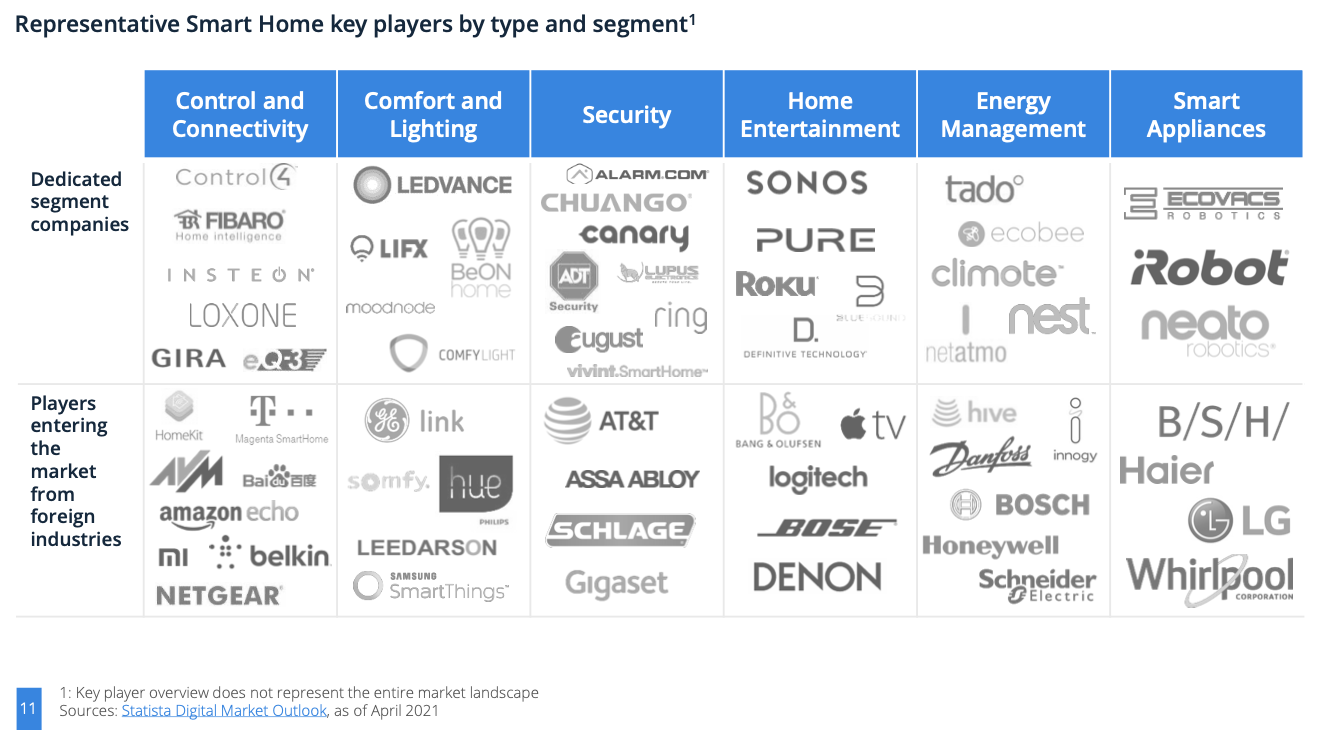
\includegraphics[width=15cm,height=10cm,keepaspectratio]{images/keyplayers.png}
            \caption{Übersicht der repräsentativen Schlüsselanbieter \cite{statista2021}} 
            \label{pic:landscape}
        \end{figure}
        \\
        Die Übersicht deckt jedoch nicht alle Anbieter ab und spezialisiert sich in diesem Fall auf die bekanntesten und die am 
        Markt etablierten. 
        \\
        \linebreak
        Laut den von Statista veröffentlichten Daten war die USA mit einem Umsatz von 28,86 Milliarden US-Dollar der größte 
        \acl{SH} Markt im Jahr 2021, wogegen Deutschland eine Umsatz von 6,59 Milliarden US-Dollar erzielte. Zu berücksichtigen sind 
        dabei jedoch die Demographische Lage als auch die Bevölkerungsdichte. Diese Aufstellung steht in keinem direkten Vergleich und 
        dient lediglich zur Veranschaulichung und zur Unterscheidung der Marktanteile. Deutlich wird dabei jedoch, dass das 
        Marktwachstum prozentual ähnlich ansteigt. 
        \\
        \linebreak
        Der Markt-Prognose in Abbildung (\ref{pic:revenue}) ist zu entnehmen, dass bis 2026 sich der Umsatz nahezu verdoppeln 
        wird. Der Darstellung (\ref{pic:globalmarket}) der einzelnen Segmente kann entnommen werden, dass der Weltmarkt von 
        2021 bis 2026 um ca. 100 Prozent zunimmt. Die Zeitspanne von 2019 bis 2026 stellt einen durchschnittlichen Zuwachs von 
        17,4 Prozent dar. Anhand der Prognose und des Berichts von Statista ist deutlich zu sehen, dass der \acl{SH} Markt in 
        den nächsten Jahren erheblich wachsen wird. Prognostiziert ist ein globaler Marktwert bei ca. 207,8 Milliarden 
        US-Dollar bis 2026.
        \begin{figure}[hbt!]
            \centering
            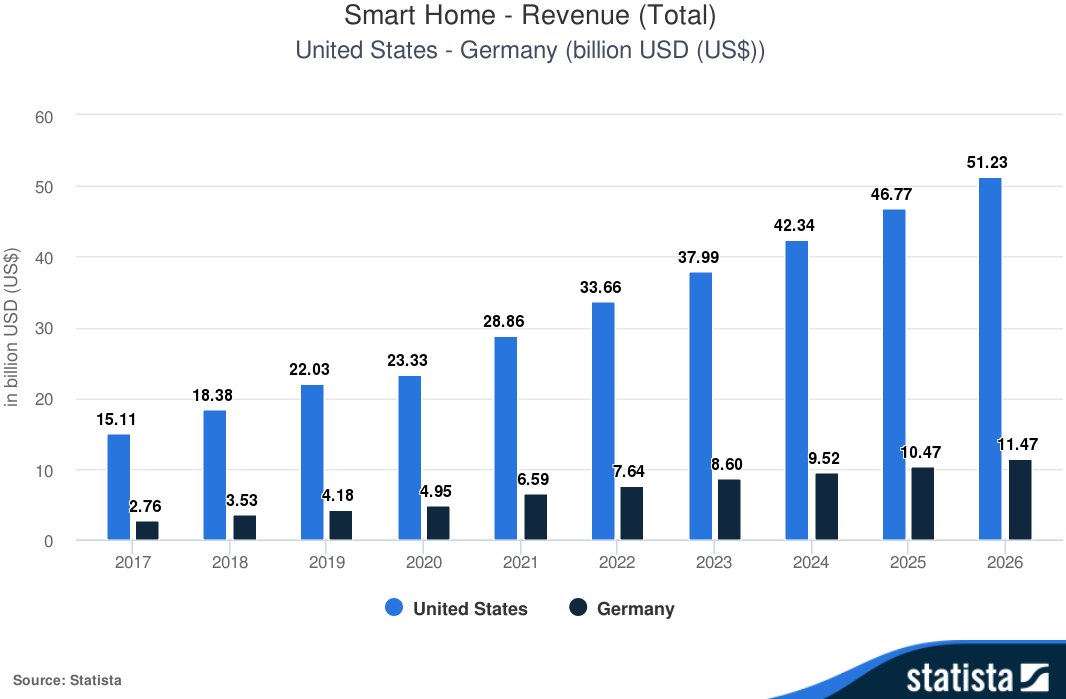
\includegraphics[width=15cm,height=9.25cm,keepaspectratio]{images/Statista-Outlook-Smart-Home---Revenue-Total-United-States---Germany-billion-USD-US.png}
            \caption{Umsatz-Prognose von Deutschland und den USA \cite{statista2021}} 
            \label{pic:revenue}
        \end{figure}
        \\
        \begin{figure}[hbt!]
            \centering
            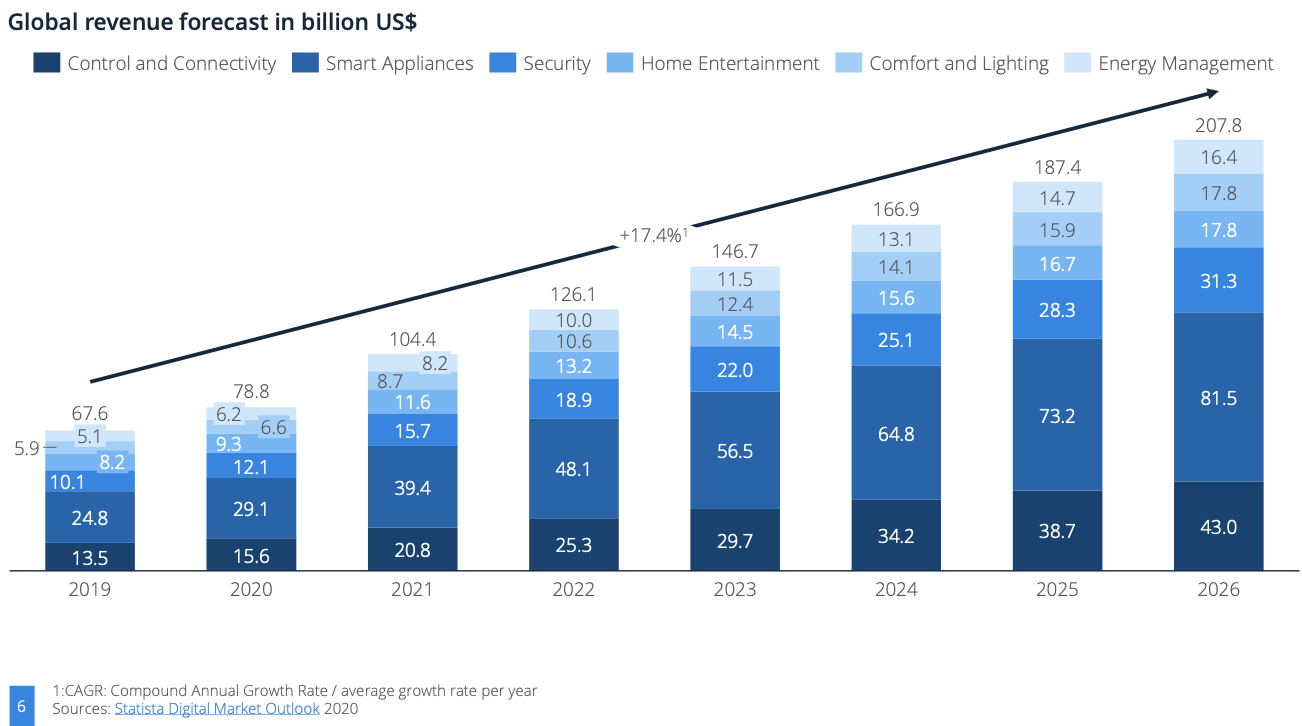
\includegraphics[width=15cm,height=10cm,keepaspectratio]{images/global_Worth_smart-home.png}
            \caption{Globaler Smart Home Marktwert \cite{statista2021}} 
            \label{pic:globalmarket}
        \end{figure}
        \pagebreak 
    \subsection*{Schlüsseltechnologien und Barrieren}
        Unter den Schlüsseltechnologien im \acl{SH} sind Komponenten zu verstehen, die den Gedanken eines intelligenten 
        Wohnraumes und Gebäudes forcieren. Dazu zählen unter anderem die Spracherkennung, die bei Sprachassistenten, 
        darunter bspw. Amazon Alexa, Apple HomePod (Siri) und dem Google Nest, eingesetzt wird, sowie \ac{AI} und \ac{KI} 
        zur Analyse, Auswertung und Optimierung von Verhaltensmustern und weiteren Analysezwecken \cite{statista2021}. 
        Obwohl die Spracherkennung das Wachstum des Marktes ankurbelt, werden die herkömmlichen Interaktionsmöglichkeiten, 
        z.B. die Kontrolle über Berührung durch Touch-Displays,
        weiter bestehen und weiterhin eine wichtige Art des Gerätezugriffs darstellen \cite{all-electronics2022}. 
        Mit dem Einsatz von \acs{KI} und \acs{AI} werden Prozesse noch autonomer und können den Komfort aus den Analysen je 
        nach Bedürfnis individuell gestalten. Zu berücksichtigen ist dabei jedoch die dafür geeigneten Anwendungsfälle und 
        die Bereitschaft der Nutzer, in wie fern diese das Analysieren von Verhaltensmustern akzeptieren und zulassen. 
            
        \subsubsection*{Fehlender Interoperabilität}
            Die Kommunikation von \acl{SH} Geräten findet über drahtlose Netzwerke auf Brandbreiten statt, die oft nicht 
            miteinander kompatibel sind. Der hauptsächliche Grund dafür ist, dass Unternehmen ein Protokoll für einen 
            bestimmten Zweck entwickeln und dieses darauf abgestimmt ist den Anwendungsfall abzudecken und um eine 
            Markteintrittsbarriere zu schaffen, sodass der Wechsel zwischen Anbietern erschwert wird \cite{statista2021}. 
            Die damit einhergehende Schwachstelle eines \acl{SH} ist, dass die Geräte mit den bereits entwickelten 
            Protokollen genutzt werden. So ist die Kommunikation über verschiedene Protokollen nicht vorgesehen. Dadurch 
            entsteht die fehlende Interoperabilität, die der Anwender jedoch für eine \acl{SH} Lösung ansieht und auch 
            als äußerst sinnvoll betrachtet. Die Einführung von Bluetooth LE Mesh ist eine aktuelle Entwicklung, um der 
            Herausforderung der Bewältigung der Interoperabilität einen Schritt näher zu kommen. Dennoch muss der 
            Anwender prüfen, welche Geräte miteinander kompatibel sind \cite{statista2021}. Bei cloudbasierten 
            Sprachdiensten muss ebenso die Kompatibilität geprüft werden. 
            Dadurch wird dem Nutzer neben der Ungewissheit der Datensicherheit und der Privatsphäre ein weiterer Aspekt 
            geliefert, der die Nutzung von \acl{SH} Lösungen für bestimmte Anwendergruppen immer noch in Frage stellt.
            \\ 
            \linebreak
            Derzeit häufig verwendete Protokolle sind unter anderem Bluetooth, \ac{WLAN} (WiFi), KNX, ZigBee, Z-Wave, 
            MQTT und weitere (siehe \ref{tab:protocolsSH}). Um Beispielsweise mit ZigBee über \acs{MQTT} kommunizieren zu 
            können, gibt es ein Framework, welches die Interoperabilität der beiden Protokolle ermöglicht. Dies ist das 
            sogenannte \textit{ZigBee2MQTT} Framework\footnote{Erschafft eine Brücke zwischen ZigBee und MQTT. \url{https://www.zigbee2mqtt.io/} Abgerufen am 23.05.2022}.
\pagebreak
\section{Zielgruppenanalyse}
\label{sec:zielgruppenanalyse}
    Zur Analyse der Zielgruppen, die \acl{SH} Lösungen nutzen, bzw. die als Anwender des im Rahmen dieser Arbeit 
    entstehenden Konzeptes gelten, erfolgt in diesem Abschnitt eine Zielgruppenanalyse. Hierbei wird zwischen 
    zwei Gruppen stark differenziert. Zum einen erfolgt die Benutzer-Analyse, die aufzeigt, welche Zielgruppen 
    im allgemeinen Kontext \acl{SH} adressiert werden, und zum anderen die Anwender-Analyse, die sich 
    konkret der Zielgruppe widmet, die in dieser Arbeit adressiert wird. 

    \subsection{Ziel der Zielgruppenanalyse}
        %was soll damit erzielt werden?
        Ziel einer Zielgruppenanalyse\footnote{Beschreibung der Zielgruppenanalyse und mögliche Durchführungsschritte. \url{https://www.eology.net/magazine/target-group-analysis} Abgerufen am 24.05.2022.} 
        ist die Identifizierung der Personengruppen, die als potentielle Nutzer eines Produktes 
        oder eines Marktsegmentes gelten. Diese Methodik ist ein relevantes Werkzeug in der Produktkonzeption und -entwicklung 
        als auch in der Marktforschung. Maßnahmen und Anforderungen können aus der Zielgruppenanalyse abgeleitet und 
        erarbeitet werden. 
        \\
        Ein Weiteres Ziel ist das bessere Kennenlernen der Zielgruppe, um dadurch deren Bedürfnisse und Interessen 
        genauer zu identifizieren und zu betrachten. 
    
    \subsection{Zielgruppe Benutzer}
        % Smart Home - Deutschland. Zugriff: 11. Mai 2022. https://de.statista.com/outlook/dmo/smart-home/deutschland
        Die in der Marktanalyse (\ref{sec:marktanalyse}) identifizierten Segmente werden in der Abbildung 
        (\ref{pic:segments}) nochmals aufgegriffen. Hierbei wird in der repräsentativen Statistik und Prognose der 
        Statista GmbH die Nutzung des jeweiligen Segments veranschaulicht. Der Fokus dieser Prognose liegt 
        auf der verstärkten Vertretung eines Segments in einem \acl{SH} in Deutschland. Die derzeit am meisten eingesetzten 
        Segmente sind \textit{Vernetzung und Steuerung} (rot gekennzeichnet) und \textit{Komfort und Licht} 
        (gelb gekennzeichnet). Das am wenigsten genutzt Segment stellt die \textit{Gebäudesicherheit} 
        (schwarz gekennzeichnet) in der Prognose dar. Im Jahr 2021 lag die Nutzung von Geräten des Segments \textit{Vernetzung 
        und Steuerung} bei 6,6 Millionen Nutzer, dicht gefolgt von dem Segment \textit{Komfort und Licht} mit 
        6,5 Millionen Nutzer. Dagegen liegt das Segment \textit{Home Entertainment} im Jahr 2021 bei 3,8 Millionen Nutzer.
        \\
        \linebreak
        Die bis 2026 veröffentlichte Prognose gibt vor, dass die jeweiligen Segmente stark zunehmen %werden 
        und sich jeweils vervierfachen.  
        \pagebreak
        \begin{figure}[hbt!]
            \centering
            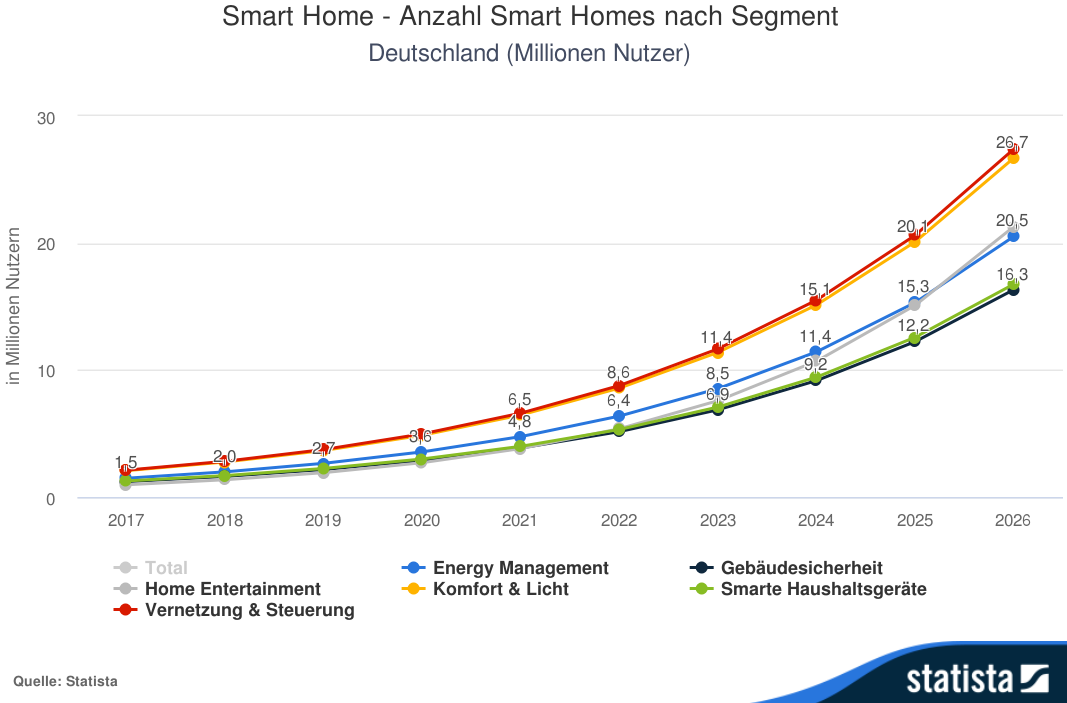
\includegraphics[width=15cm,height=10cm,keepaspectratio]{images/Statista-Outlook-Smart-Home---Anzahl-Smart-Homes-nach-Segment-Deutschland-Millionen-Nutzer.png}
            \caption{Anzahl Smart Home nach Segment \cite{statista2021}} 
            \label{pic:segments}
        \end{figure}
        \\
        Das Resümee der Prognose zeigt, dass eine breitere Masse an Personen bereits Komponenten der Segmente 
        \textit{Vernetzung und Steuerung} und \textit{Komfort und Licht} nutzen.
        \\
        \linebreak
        Im Hinblick auf die demographischen Statistiken wird in der Zielgruppenanalyse deutlich, welche Gesellschaftsschicht 
        im Jahr 2021 am stärksten vertreten ist. Diese erstreckt sich über eine Altersspanne von 25 bis 54 Jahren. 
        Wobei der Abbildung (\ref{pic:ageSH}) zu entnehmen ist, dass der Schwerpunkte im Alter zwischen 45 und 54 Jahren 
        mit 22,7 Prozent. Die Balance nach Geschlecht liegt bei einem Anteil von 45,6 Prozent weiblichen Befragten und 
        54,4 Prozent männlichen Befragten, demnach eine geringe Ungleichheit. Die Auswertung nach Einkommen zeigt, dass 
        35,4 Prozent der Befragten mit mittlerem Einkommen Komponenten eines \acl{SH} nutzen, dicht gefolgt von 
        Personen mit hohem Einkommen, diese liegen bei 34,9 Prozent. 
        \\
        \linebreak
        Demzufolge ist eine große Masse adressiert, die jedoch nach den Segmenten (siehe Abbildung \ref{pic:segments}) 
        wiederum eingeschränkt werden kann.
        \pagebreak
        \begin{figure}[hbt!]
            \centering
            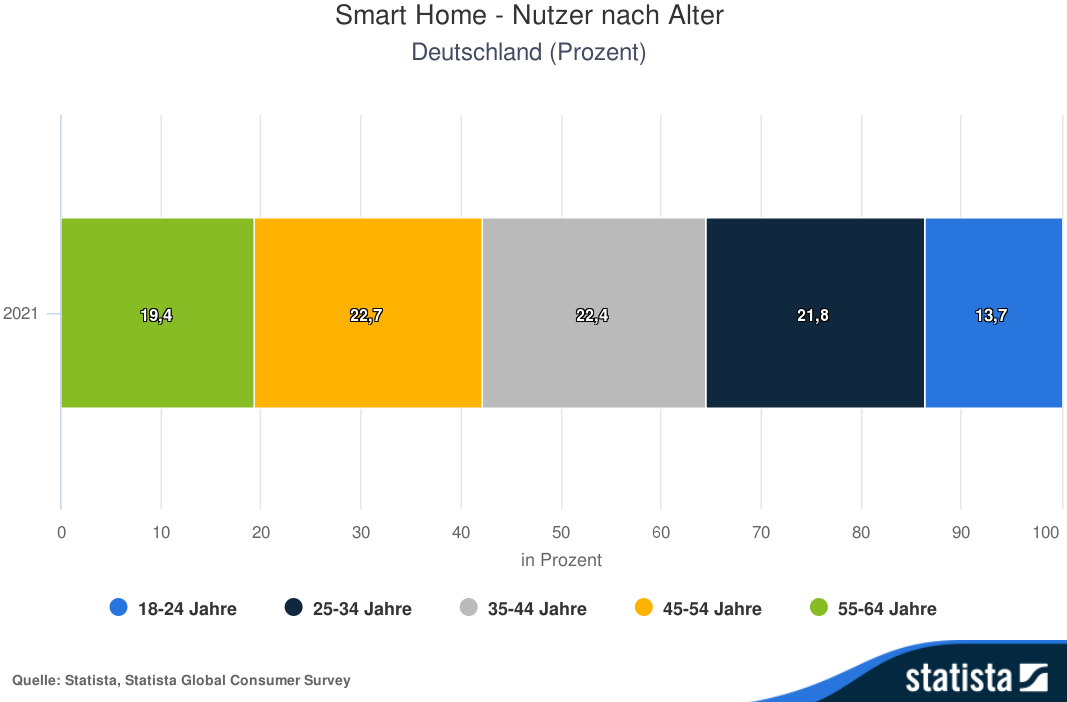
\includegraphics[width=15cm,height=10cm,keepaspectratio]{images/Statista-Outlook-Smart-Home---Nutzer-nach-Alter-Deutschland-Prozent.png}
            \caption{Smart Home Nutzer nach Alter \cite{statista2021}} 
            \label{pic:ageSH}
        \end{figure}
        \\
        Die aufgeführten Statistiken und Prognosen zeigen den Markt rundum \acl{SH} auf und welches Potential für die 
        nächsten Jahre prognostiziert wird. Im Hinblick auf die Zielgruppe lässt sich sagen, dass eine breite Masse 
        fokussiert werden kann, die jeweils unterschiedliche Voraussetzungen und Bedürfnisse haben. Diese Analyse zeigt 
        jedoch den gesamten Markt auf, um einen Einblick zu gewährleisten, wie stark \acl{SH} momentan in Deutschland, den 
        Vereinigten Staaten (USA) und dem Rest der Welt vertreten ist. Um einen konkreteren Einblick 
        zu gelangen, wird in nachfolgendem Abschnitt auf die Zielgruppe der Anwender, die in dieser Arbeit fokussiert werden, 
        eingegangen. 

    \subsection{Zielgruppe Anwender}
        %Die eigentliche Zielgruppe, die Softwareentwickler, die das System betreiben und für ihre Bedürfnisse anpassen.
        Der Benutzergruppe wird die Anwenderzielgruppe gegenübergestellt, diese können jedoch ebenso Benutzer der Anwendung 
        werden. Im Umkehrschluss ist ein gewisses Maß an \acs{IT}-Affinität vorausgesetzt, sodass Benutzer nicht gleich 
        Anwender sein können. Es wird eine grundlegende Kenntnis der Programmierung erfordert, im Rahmen dieser Arbeit 
        der Umgang mit der Programmiersprache Java. Einer Umfrage der Developer Nation\footnote{Umfragen, Statistiken und Berichte rundum Softwareentwickler\url{https://www.developernation.net/developer-reports/dn21} Abgerufen am 27.05.2022} 
        zufolge, benutzen von ca. 12.5 Tausend Befragten im Jahr 2021 35.8 Prozent die Programmiersprache Java. Somit kann 
        ein Rückschluss erfolgen, dass Java eine der am häufigsten verwendete Programmiersprache ist.
        \\
        \linebreak
        Im Fokus der Arbeit steht der Softwareentwickler als Anwender, welcher das System betreibt und auf die 
        individuellen Bedürfnisse anpasst. 
        \\
        Laut des Berichts der Developer Nation\footnote{Umfragen, Statistiken und Berichte rundum Softwareentwickler\url{https://www.developernation.net/developer-reports/dn21} Abgerufen am 27.05.2022}
        des dritten Quartals 2021 gibt es zu diesem Zeitpunkt 26.8 Millionen Softwareentwickler weltweit. Davon sind dem 
        Bericht von Daxx\footnote{Zusammenfassung mehrerer Berichte. \url{https://www.daxx.com/de/blog/entwicklungstrends/anzahl-an-softwareentwicklern-deutschland-weltweit-usa} Abgerufen am 27.05.2022}
        zufolge 0.9 Millionen in Deutschland angesiedelt. 
        \\
        \linebreak
        Eine vergleichbare Anwendergruppe ist die der Softwarelösung openHAB. Diese ist weltweit bekannt und zählt unter die 
        beliebtesten und am meist genutzt open source Lösungen. Anhand den eigenen Statistiken kann die Community\footnote{Website Statistik der openHAB Community. \url{https://community.openhab.org/about} Abgerufen am 27.05.2022} 
        der openHAB Foundation ca. 42 Tausend Benutzer und Anwender vorweisen. Dem GitHub Repository der \textit{openhab-core} 
        Software sind 73 Mitwirkende zugeschrieben, die dazu beitragen die Software weiterzuentwickeln, bzw. zu verbessern und zu 
        stabilisieren.
    \\
    \linebreak 
    Damit die adressierte Zielgruppe etwas greifbarer wird und die Anwendungsschritte der \textit{target group analysis} und 
    dem \textit{user-centered design} eingehalten werden, sind Persona\footnote{Eine repräsentative Vorstellung einer Person zu bestimmtem Kontext. \url{https://www.romanpichler.com/the-persona-template/} Abgerufen am 28.05.2022} 
    entwickelt worden. Diese geben die Anwenderzielgruppe wieder und geben einen Eindruck über die Personen, die sich mit dem 
    Softwareprodukt, bzw. mit dem Konzept auseinandersetzen. Die entstandenen Persona sind dem Anhang beigefügt 
    (siehe REFERENZ TBD). %\ref{}

\section{Anwendungsfälle - Use Cases}
\label{sec:usecases}
    Für die Erhebung und Ausarbeitung von Anforderungen an die einfache Handhabung der formalisierten 
    Interaktionen des Softwareentwicklers zur Erweiterung des Systems und dessen Regeldefinitionen werden Anwendungsfälle, 
    sogenannte Use Cases, definiert, bewertet und auf ihre Funktionalität geprüft. Diese wurden im Rahmen 
    des \acl{RE} dokumentiert. Das \acs{RE} nach \cite{pohl2021basiswissen} gibt Schablonen, Vorgehensmodelle und Aufgaben 
    vor, die dabei helfen, den Kontext des Projektes zu erläutern und aus den anliegenden Sachverhalten und Anwendungsfällen 
    die Anforderungen abzuleiten. Nach der strukturierten \acs{RE} Methode \ac{TORE} \cite{tore2014} werden die 
    Aufgaben, die Systemfunktionen und die Interaktionen deutlich. Zum besseren Verständnis des Kontextes und der daraus 
    resultierenden Anforderungen werden die jeweils generierten Anwendungsfälle in den folgenden Abschnitten 
    erläutert.
    \\
    \linebreak
    %Zum besseren Verständnis wird auf diese in den folgenden Abschnitten eingegangen. 
\subsection{Check In mit einem Service-Roboter}
    Der Anwendungsfall des Check Ins mit einem Service-Roboter skizziert das Szenario und den Kontext des Sachverhaltes, als 
    auch die Komponenten, die benötigt werden, um den grundlegenden Aufbau der Regeldefinition und -implementierung sowie 
    der Steuerzentrale darzustellen. Daran sind die Bausteine und Anforderungen zu entnehmen, die für das Konzept notwendig 
    sind. Anhand dessen können die Schritte des Anwenders identifiziert werden, die notwendig sind, um die Interaktionen für den 
    Softwareentwickler zu identifizieren und so zu verallgemeinern, dass die formalisierten Interaktionen einfach zu 
    handhaben sind. Des weiteren soll durch die Komplexität der Anwendungsfälle auch ersichtlich werden, welche fundamentalen 
    Komponenten und Konzeptentscheidungen notwendig sind, damit über die Steuerzentrale solche Anwendungsfälle abgebildet werden 
    können.
    \\
    \linebreak
    Der Check In erfordert drei Teilnehmer und eine vorausgesetzte Bedingung, die bereits implementiert ist. Als Teilnehmer 
    zählt eine Person, die den Check In erfährt, ein Service-Roboter, der die Begrüßung und das Check In als Anweisung 
    durchführt und die Steuerzentrale, die den Ablauf koordiniert. Als bereits implementierter Vorgang wird die 
    Authentifizierung der Person über eine Kamera an der Eingangstür vorausgesetzt. Diese veröffentlicht nach erfolgreicher 
    Authentifizierung eine Nachricht an einen Nachrichten-Broker. An dieser Stelle hört die Steuerzentrale auf die 
    veröffentlichte Nachricht und konsumiert diese. Mit dem Ereignis ist der Auslöser für die weiteren Schritte gegeben. Nach 
    dem Erhalt der Nachricht wird diese zugeordnet und die dafür vorgesehene Regel angestoßen. Mit Beginn der Anweisung wird 
    der Service-Roboter an die Tür geschickt, um die Person zu begrüßen. Parallel dazu wird über eine Schnittstelle zu einer 
    internen Software zur Büroplatzbuchung abgefragt, ob die authentifizierte Person bereits einen Büroplatz gebucht hat. 
    Die Information wird in weiterem Schritt für den Check In benötigt. Sobald der Service-Roboter an der Tür angelangt ist, 
    öffnet sich diese und die Person kann eintreten. Wenn die zu begrüßende Person vor dem Service-Roboter steht, kann dieser 
    mithilfe einer integrierten Kamera erkennen, dass eine Person gegenübersteht. Zu diesem Zeitpunkt wird zur Einfachheit 
    damit gerechnet, dass die Person, die vor dem Service-Roboter steht auch diejenige ist, die an der Tür authentifiziert 
    wurde. In zukünftiger Arbeit könnte die Person auch über die Kamera des Roboters erneut authentifiziert werden, damit die 
    Korrektheit gegeben ist. Dies ist zu diesem Anwendungsfall jedoch nicht erforderlich und wird deshalb an dieser Stelle 
    nicht weiter verfolgt. 
    \\
    Nachdem der Roboter die Person erkannt hat, startet die formale Begrüßung. Anschließend wird die Information der 
    vorherigen Büroplatzbuchung verwendet, um das Einchecken der Person zu starten. Wurde bei der Abfrage eine Buchung für 
    die Person gefunden, so kann sich diese als anwesend einchecken und an den Arbeitsplatz gehen. Ist jedoch keine 
    Buchung gefunden worden, so kann ein freier Platz über den Roboter reserviert, bzw. gebucht werden. Die Buchung wird 
    anschließend an die Steuerzentrale zurückgegeben und über diese in das Buchungsportal eingepflegt. Nachdem dieser 
    Schritt abgearbeitet ist, endet der Anwendungsfall und der Service-Roboter wird an seine Ausgangsposition, bzw. an dessen 
    Ladestation geschickt. Somit ist das Szenario abgearbeitet und der Roboter steht für weitere Aufgaben zur Verfügung. 
    \\
    \linebreak
    Zur besseren Veranschaulichung des Anwendungsfalls sind im Anhang (%\ref{}%
    SIEHE REFERENZ TBD) eine weitere Aufgabenbeschreibung, sowie die User Story als auch ein Use Case-, 
    Sequenz- und Ablaufdiagramm zu finden.

\subsection{Notfall-Evakuierung mit einem Service-Roboter}
    Mit dem Szenario der Notfall-Evakuierung wird ein weiterer Anwendungsfall definiert, welcher dabei helfen soll, die 
    Anforderungen zu identifizieren, die für die Bereitstellung des Frameworks der Steuerzentrale benötigt werden.
    Objektiv betrachtet gibt es bei diesem Fall ebenso einen Auslöser, als Beispiel einen Sensor, bspw. einen Rauch- 
    oder Gasmelder, der eine Nachricht veröffentlicht, die über die Steuerzentrale konsumiert, verarbeitet und dadurch die 
    weiteren notwendigen Schritte eingeleitet werden. Nachdem die Nachricht von der Steuerzentrale erhalten wurde, wird 
    darauf basierend die Regel und die darauffolgende Aktion angestoßen. Die Steuerzentrale muss über die \acs{API} 
    Schnittstelle des internen Büroplatzbuchungssystems alle eingecheckten Personen und Platzbuchungen abfragen und 
    zwischenspeichern. Die Informationen werden genutzt, um den Service-Roboter an die Arbeitsplätze der jeweilig 
    eingecheckten Personen zu schicken, sodass dadurch diese über den Notfall informiert, bzw. gebeten werden, das 
    Gebäude zu verlassen. Wird eine Person an einem Arbeitsplatz erkannt, so kann diese über den Sachverhalt informiert 
    werden. Ist jedoch der Arbeitsplatz leer, soll der Service-Roboter den nächsten Arbeitsplatz ansteuern. Nachdem alle 
    Plätze von dem Service-Roboter abgefahren wurden, soll dieser über die restliche Bürofläche fahren und nach Personen 
    suchen. Die Erkennung der Person wird durch die Kamera des Roboters durchgeführt. Abschließend, wenn alle Plätze und die 
    Bürofläche abgefahren wurden, soll der Roboter an eine zentrale Stelle im Büro fahren und ohne Unterbrechung eine 
    Durchsage starten und diese solange wiederholen, bis eine Person den Vorgang beendet. Mit der Beendung der Dauerschleife 
    ist das Szenario abgeschlossen und der Roboter kann an seine Ausgangsposition zurückgeführt werden, sofern dies 
    umgebungsbedingt noch möglich ist.
    \\
    Somit ist der zweite Anwendungsfall definiert. Die textuelle Schilderung des Szenarios wird mit im Rahmen des \acs{RE} 
    vorgesehenen Diagrammen und Visualisierungen gestützt. Diese sind dem Anhang (%\ref{}%
    SIEHE REFERENZ TBD) zu entnehmen.
    \\
    \linebreak
    Die Anwendungsfälle wurden so gewählt, da diese eine gewisse Komplexität mit sich bringen, die es mit der Steuerzentrale 
    abzudecken gilt.
    \\
    Aus dem Kontext beider Anwendungsfälle, der vorangestellten Zielgruppenanalyse und den Experteninterviews werden in Abschnitt 
    (\ref{sec:requirementsFinal}) die daraus identifizierten Anforderungen für die Steuerzentrale aufgeführt.

\section{Experteninterview}
\label{sec:experteninterviewReqirements}
    Zur Analyse und Erhebung von Anforderungen, die sich an das System richten, werden Experteninterviews durchgeführt. 
    Dabei wird sich, wie in dem Abschnitt (\ref{subsec:experteninterview}) beschrieben, an dem unstrukturierten Ansatz der 
    Führung eines solchen Interviews orientiert \cite{robson2002real}. Infolgedessen werden keine konkreten offenen oder 
    geschlossenen Fragen gestellt. Der Aufbau des Interviews wird in weiteren Schritten aufgegriffen. 
    \\
    Die Ergebnisse der Interviews sind nicht repräsentativ, da sie im Rahmen dieser Arbeit keine große Masse abdecken. Diese 
    dienen lediglich der weiträumigeren Informationsgewinnung und dem Sammeln mehrerer Meinungsbilder, um aus allen 
    Ideen, Gedankenanstößen und Meinungen ein objektives Gesamtbild zu erzeugen und daraus viele Anforderungen zu gewinnen 
    und abzuleiten. 
    %Die Experten Interviews sind eine Möglichkeit, die Anforderungen zu erfassen, die durch die Entwicklung des Systems 
    %nicht durch eine einfache Marktanalyse erfasst werden konnten. Diese Interviews sind nicht repräsentativ und dienen lediglich 
    %der weiträumigeren Informationsgewinnung.
\subsection{Ziel des Experteninterviews}
    % Diese helfen dabei, mehrere Sichten, Meinungen und Erfahrungen einzuholen, um ein 
    Ziel des Experteninterview ist die Informationsgewinnung aus bestimmten Sachverhalten, die nicht leicht auf anderem Wege 
    zu beschaffen sind. Der Experte dient als Informationsträger und kann dabei helfen seine Sicht auf den Sachverhalt 
    wiederzugeben. Dadurch können Meinungen eingeholt und Erfahrungen ausgetauscht werden. Diese sind oft wichtige 
    Informationen zur Erhebung von Anforderungen einem bestimmten Sachverhalt gegenüber.

\subsection{Aufbau des Experteninterviews}
    Die Experteninterviews wurden im Gesamten als unstrukturierte Interviews durchgeführt. Lediglich die Rahmenbedingungen sowie 
    der Einstieg in das Interview waren vorgegeben und bei jeder interviewten Person ähnlich. Zu Anfang des Gesprächs wurde 
    der Kontext und die Intension erläutert, damit der Experte die Situation und die Absichten kennen lernt und die 
    eigentliche Herausforderung %Problemstellung%
    erkennt. Grundlage dafür war die Erläuterung der Zielsetzung (\ref{sec:zielsetzung}) der Arbeit, 
    um so die Intension zu verdeutlichen. Mit den identifizierten Anwendungsfällen (\ref{sec:usecases}), die als Basis 
    zur Extraktion von Anforderungen und als potentiell umsetzbare Funktionalitäten gelten, wurden Szenarien veranschaulicht, 
    die dabei halfen, das Anwendungsumfeld zu konkretisieren.  
    Nach der Schilderung des Kontextes und der zugrundeliegenden Ausgangspunkten wurde das Gespräch in Richtung Anforderungen 
    gelenkt. Hierbei lag der Fokus auf der Erhebung der Ideen, Sichtweisen und Meinungen, die als Grundlage für Anforderungen 
    dienten oder gar direkte Anforderungen an das System ergaben. Dabei war der Ausgang des Gesprächs offen. Falls während 
    eines Gespräches der Fokus verloren ging, bzw. Exkurse ein zu großes Ausmaß annahmen, wurde wieder auf die 
    vorliegende Sachlage aufmerksam gemacht und der Fokus erneut auf die Anforderungen geworfen. 
    Schwerpunkte bei den Interviews waren zum einen, welche Anforderungen gelten, um eine einfache Handhabung der 
    formalisierten Interaktionen für den Softwareentwickler zu gewährleisten und zum anderen die Funktionalitäten, die der 
    Experte dem System gegenüber sieht, um ein Regelwerk für ein intelligentes Büro zu erstellen. 
    Ebenso wurden nichtfunktionale Anforderungen, die ein solches System mit sich bringen soll, adressiert. 
    Die zusammengefassten Anforderungen und daraus abgeleiteten Bedingungen sind dem Abschnitt (\ref{sec:requirementsFinal}) 
    zu entnehmen.
    % Zum Einstieg des Interviews wird der Kontext erläutert (Welche Software entwickelt werden soll) UND 
    % dass der Fokus auf der einfachen Handhabung der formalisierten Interaktionen für SOFTWAREENTWICKLER liegt. 
    % Welche Anforderungen der Experte in der Funktionalität als auch Anforderungen dem System gegenüber sieht. 
     
\subsection{Zusammenfassung der Experteninterviews}
    %TODO: Anzahl der Interviews ggf. anpassen (mehrere angeben)
    In Summe wurden insgesamt vier Experteninterviews durchgeführt. Jedes Gespräch war individuell und hatte dementsprechend 
    einen anderen Verlauf, bzw. ein anderes Ergebnis. Dennoch konnte der inhaltliche Fokus gewahrt und verschiedene 
    Meinungsbilder eingeholt werden. Jeder befragte Experte konnte zu dem anliegenden Sachverhalt seine Meinung äußern und 
    wichtige Informationen und Sichtweisen mitteilen. Die erhobenen Informationen wurden analysiert, aufbereitet und 
    als Anforderungen dokumentiert. Die dabei entstandenen Informationen und Anforderungen werden in 
    folgendem Abschnitt aufgezeigt. 
    % Interessante Gespräche wurden geführt. Bereits die Schilderung des Kontextes und der Idee gab es Diskussionsbedarf und 
    % Anforderungen, die sehr interessant waren und als Anforderungen so mit aufgenommen worden sind. 
    % Aus den Interviews ergaben sich Anforderungen, die in die Konzeption mit einfließen. Diese werden im folgenden 
    % Abschnitt thematisiert.
    
\pagebreak
\section{Anforderungen}
\label{sec:requirementsFinal}
    In Folge der vorangestellten Literaturrecherche, der Markt- und, Zielgruppenanalyse, der entwickelten Anwendungsfälle und 
    der durchgeführten Experteninterviews ergaben sich Anforderungen an das System als auch Bausteine, die in der 
    Konzeption und der anschließenden Implementierung einer solchen Software essentiell sind. Da der Fokus dieser 
    Arbeit auf der einfachen Handhabung der formalisierten Interaktionen für den Softwareentwickler liegt, werden 
    Anforderungen, die in diese Richtung adressiert sind, höher priorisiert, als allgemeingültige Anforderungen, die mehr das 
    Verhalten einer solchen Software beschreiben. 
    \\
    Den folgenden Tabellen sind die Anforderungen zu entnehmen:
    \begin{table}[hbt!]
        \begin{center}
            \begin{tabular}{| p{10.4cm} | p{1.8cm} | p{3.2cm} | }
                \hline
                   \textbf{Anforderung} & \textbf{Priorität} & \textbf{Quelle} \\
                \hline
                    Es soll eine Struktur vorgegeben werden, mit der einfach und formell Regeln und Prozesse implementiert werden können. & Essentiell & Experteninterview \\ 
                \hline
                    Das Konstrukt von Regeln soll allgemeingültig sein, dass der Entwickler die Logik (Bedingung, Aktion \& Zusätze) implementieren muss. & Essentiell & Experteninterview \\
                \hline
                    Nachrichten und Auslöser über Nachrichten sollen empfangen und verarbeitet werden können. & Essentiell & Experteninterview, Anwendungsfall \\
                \hline
                    Es soll eine allgemeingültige Programmiersprache verwendet werden. & Mittel & Experteninterview, Zielgruppenanalyse \\ 
                \hline
                    Komponenten müssen digital abgebildet werden. & Mittel & Experteninterview, Anwendungsfall \\ 
                \hline
                    Komponenten und dessen Zustände müssen abgebildet werden. & Hoch & Experteninterview, Anwendungsfall \\ 
                \hline
                    Aktionen und Regeln sollen nach einem bestimmten Auslöser (Trigger) ausgeführt werden. & Hoch & Experteninterview, Anwendungsfall \\
                \hline
                    Aktionen sollen parallel ausgeführt werden können. & Mittel & Experteninterview \\ 
                \hline
                    Aktionen, welche die gleiche Komponente beanspruchen, sollen nacheinander ausgeführt werden können. & Mittel & Experteninterview \\
                \hline
                    Die Zustände der Komponenten sollten persistiert werden, damit bei einem Systemausfall oder -fehler diese nicht verloren gehen. & Mittel & Experteninterview \\ 
                \hline 
            \end{tabular}
        \end{center}
        \caption{Abstrakte Anforderungen}
        \label{tab:abstractRequirements}
    \end{table} 
    \\
    \begin{table}[hbt!]
        \begin{center}
            \begin{tabular}{| p{10.4cm} | p{1.8cm} | p{3.2cm} | }
                \hline
                   \textbf{Anforderung} & \textbf{Priorität} & \textbf{Quelle} \\
                \hline
                    Als Programmiersprache soll Java verwendet werden. & Mittel & Experteninterview, Zielgruppenanalyse \\ 
                \hline
                    Damit Komponenten abgebildet werden können, muss ein Zustandsraum definiert sein. & Essentiell & Experteninterview, Anwendungsfall \\ 
                \hline
                    Der Zustandsraum muss zur Laufzeit immer zur Verfügung stehen. & Hoch & Experteninterview, Anwendungsfall \\ 
                \hline
                    Regeln und darauf ausgelöste Aktionen sollen über MQTT Nachrichten oder zeitbasiert ausgelöst werden. & Hoch & Experteninterview, Anwendungsfall \\
                \hline
                    Nutzung eines Thread Pools zur parallelen Ausführung von Regeln. & Mittel & Experteninterview \\ 
                \hline
                    Aktionen, welche die gleiche Komponente beanspruchen, sollen nacheinander ausgeführt werden können. & Mittel & Experteninterview \\
                \hline
            \end{tabular}
        \end{center}
        \caption{Konkretere Anforderungen}
        \label{tab:concretRequirements}
    \end{table}
    \\
    \begin{table}[hbt!]
        \begin{center}
            \begin{tabular}{| p{7.0cm} | p{7.0cm} | p{1.4cm} | }
                \hline
                   \textbf{Funktionale Anforderung} & \textbf{Nichtfunktionale Anforderungen} & \textbf{Quelle} \\
                \hline
                    Bereitstellung eines Konstruktes zur Implementierung eines Regelsets. & Zuverlässigkeit: Durch einen Auslöser gestartete Aktionen sollen bei gleichem Auslöser immer die gleiche Aktion anstoßen. & Ex.-Interv. \\ 
                \hline
                    MQTT Nachrichten werden verarbeitet und an einen Auslöser weitergeleitet. & Die Steuerzentrale muss eine Verfügbarkeit von 99,9\% vorweisen. & Ex.-Interv. \\ 
                \hline
                    Implementierung eines MQTT Subscriber and Producer. & Die Kommunikation erfolgt ausschließlich über MQTT. & AW-Fall \\ 
                \hline
                    Speicherung des Zustandsraumes in eine Datenbanken. & Single Point of Contact (Implementierung, Anpassung und Erweiterung der Regel und der Logik). & Zielgr.-Analyse \\
                \hline
                    Erweiterungen zu API Anbindungen per MQTT. & Sicherheit: Es werden nur Schnittstellen zur Datenabfrage erlaubt. & Ex.-Interv. \\ 
                \hline
                    Abbildung von Zustandsinformationen. & Die Steuerzentrale ist nur im eigenen Netz erreichbar. & Ex.-Interv. \\
                \hline
            \end{tabular}
        \end{center}
        \caption{Funktionale und Nichtfunktionale Anforderungen}
        \label{tab:FAandNFA}
    \end{table}

    % Alle aufgeführten Anforderungen fließen mit in die Konzeption ein und bilden die Grundlage für die Ausarbeitung des 
    % Konzeptes. Das folgende Kapitel (\ref{chap:konzept}) widmet sich dem Konzept.
